\section{Үр дүн}
\subsection{Вэб сайтын нүүр хэсэг}

\begin{figure}
	\centering
	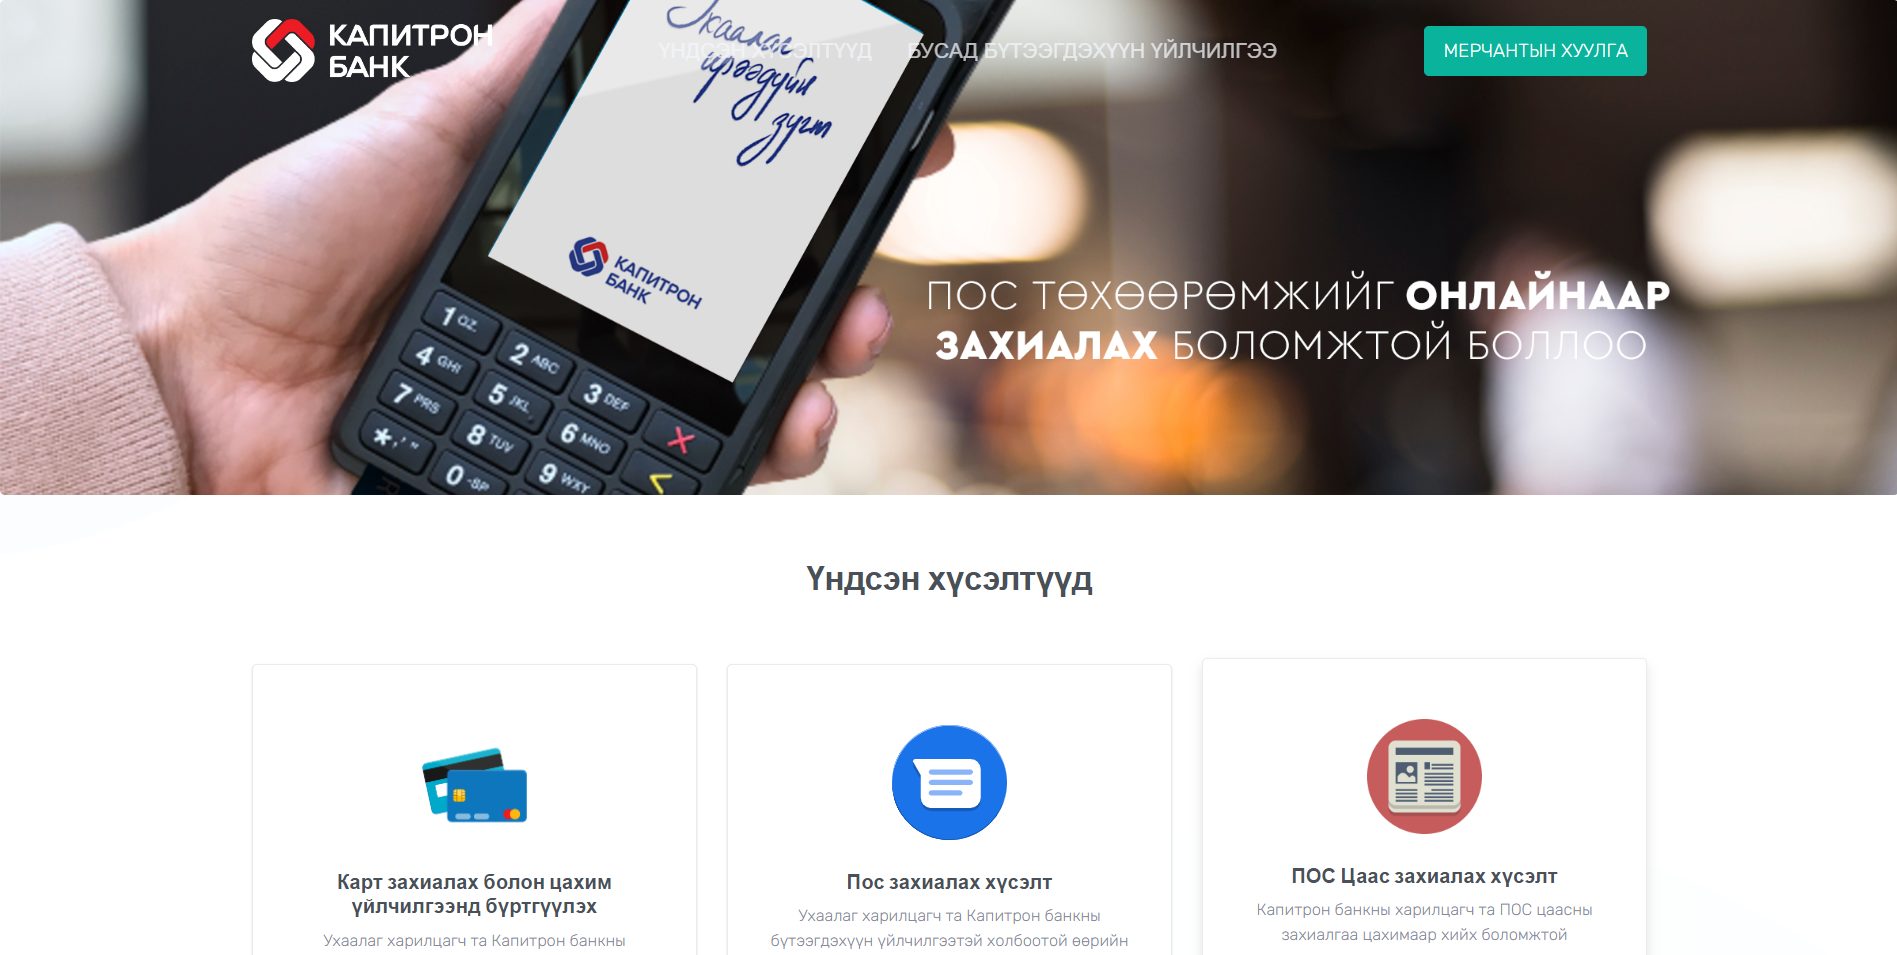
\includegraphics[width=15cm]{images/merchant.png}
	\caption{Нүүр хэсэг}
	\label{fig:homepage}
\end{figure}
\pagebreak

\subsection{Ajax ашиглан хүсэлтийг modal байдлаар гаргах}

\begin{figure}
	\centering
	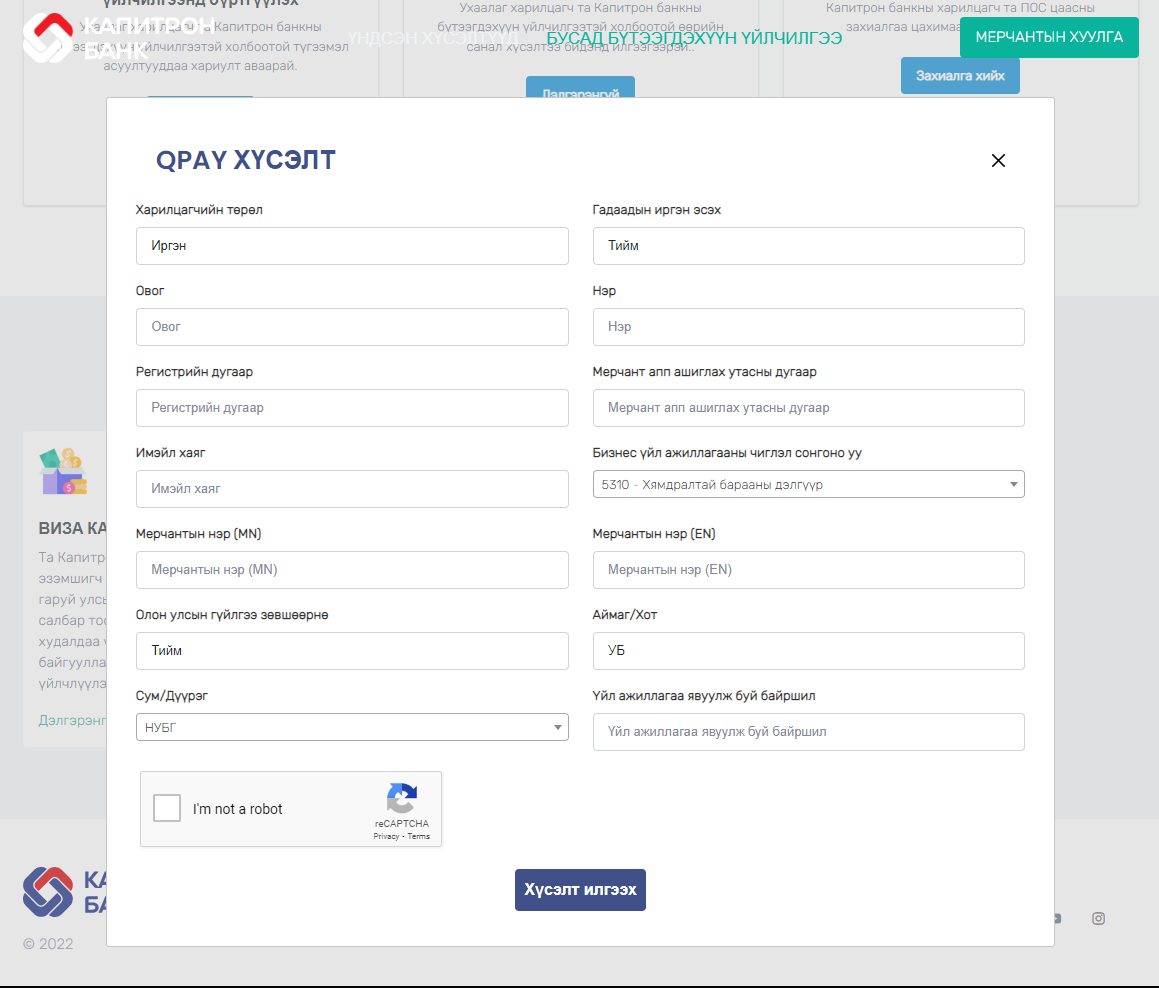
\includegraphics[width=14cm]{images/qpay_form.png}
	\caption{Qpay хүсэлт}
	\label{fig:modalform}
\end{figure}
\pagebreak

\subsection{Байгууллагуудын лого}
\begin{figure}
	\centering
	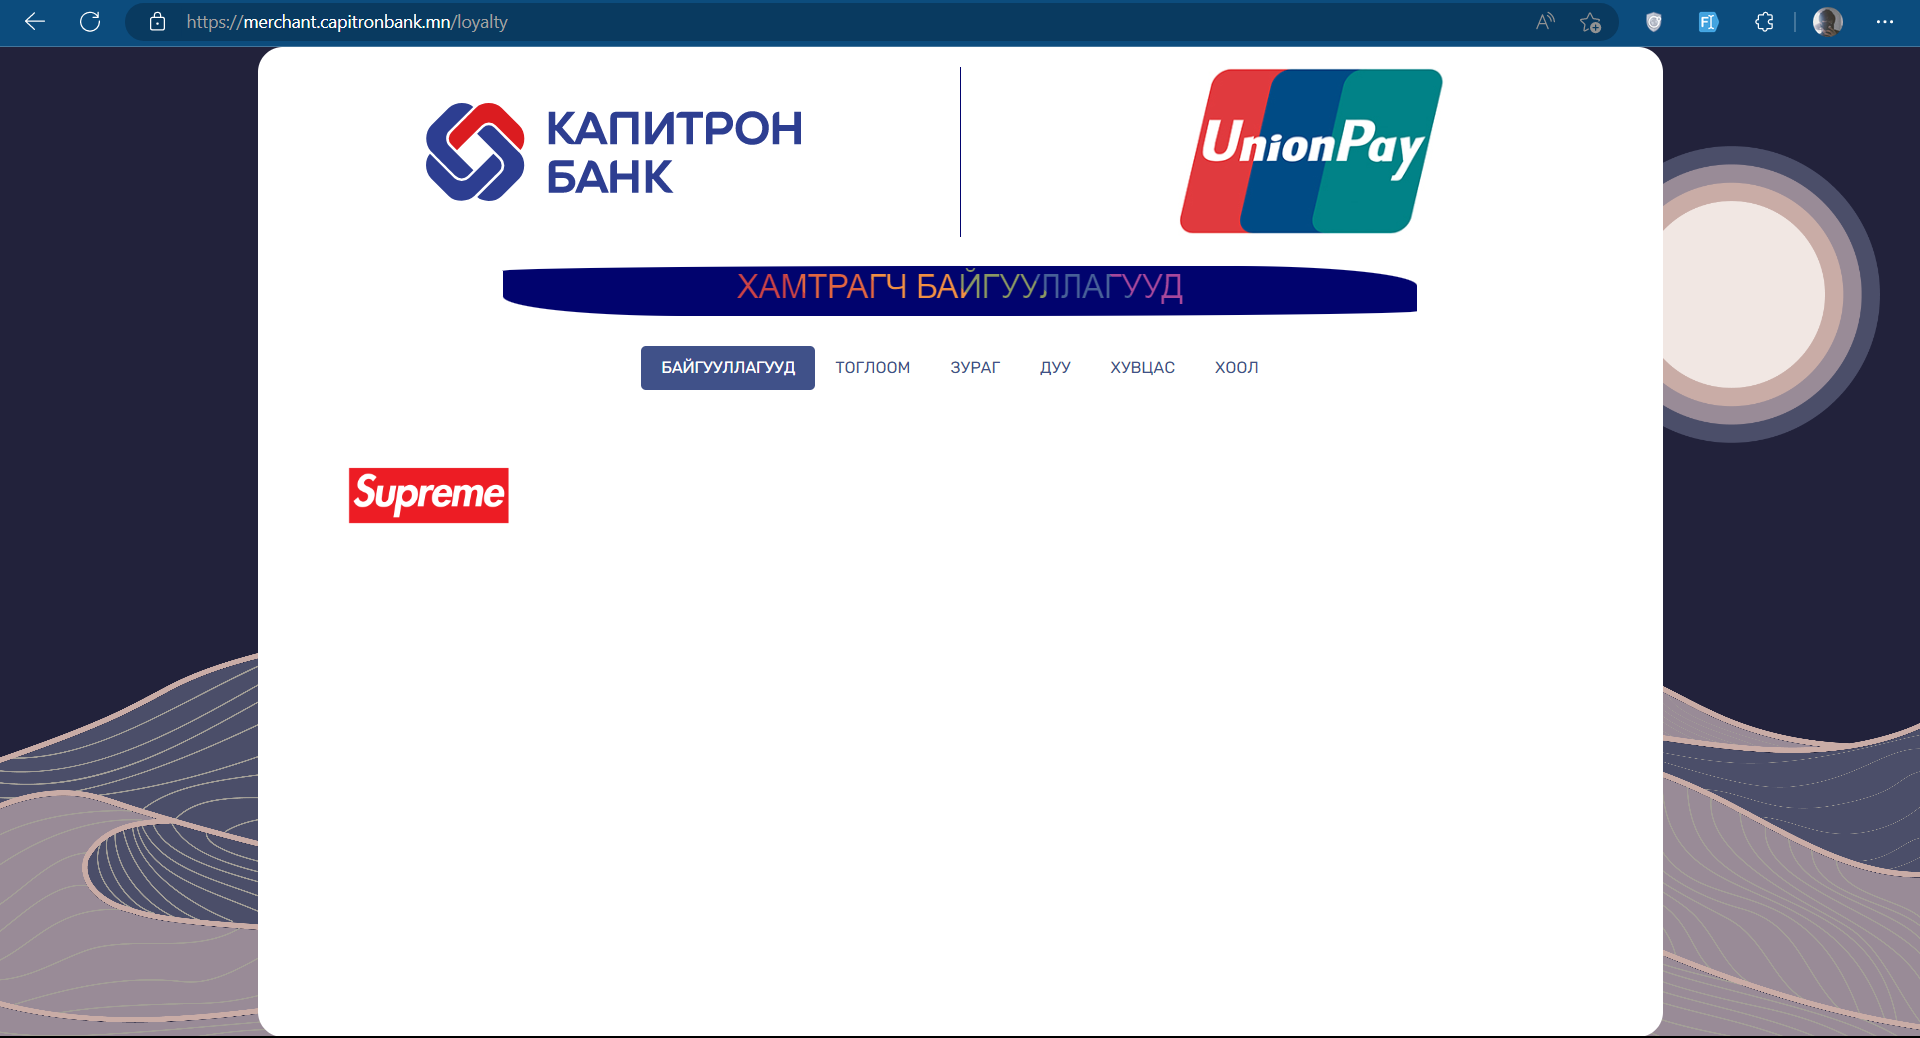
\includegraphics[width=14cm]{images/loyalty.png}
	\caption{Merchant Loyalty хэсэг}
	\label{fig:toast}
\end{figure}
\pagebreak

\subsection{Админ CRUD хэсэг}
\begin{figure}
	\centering
	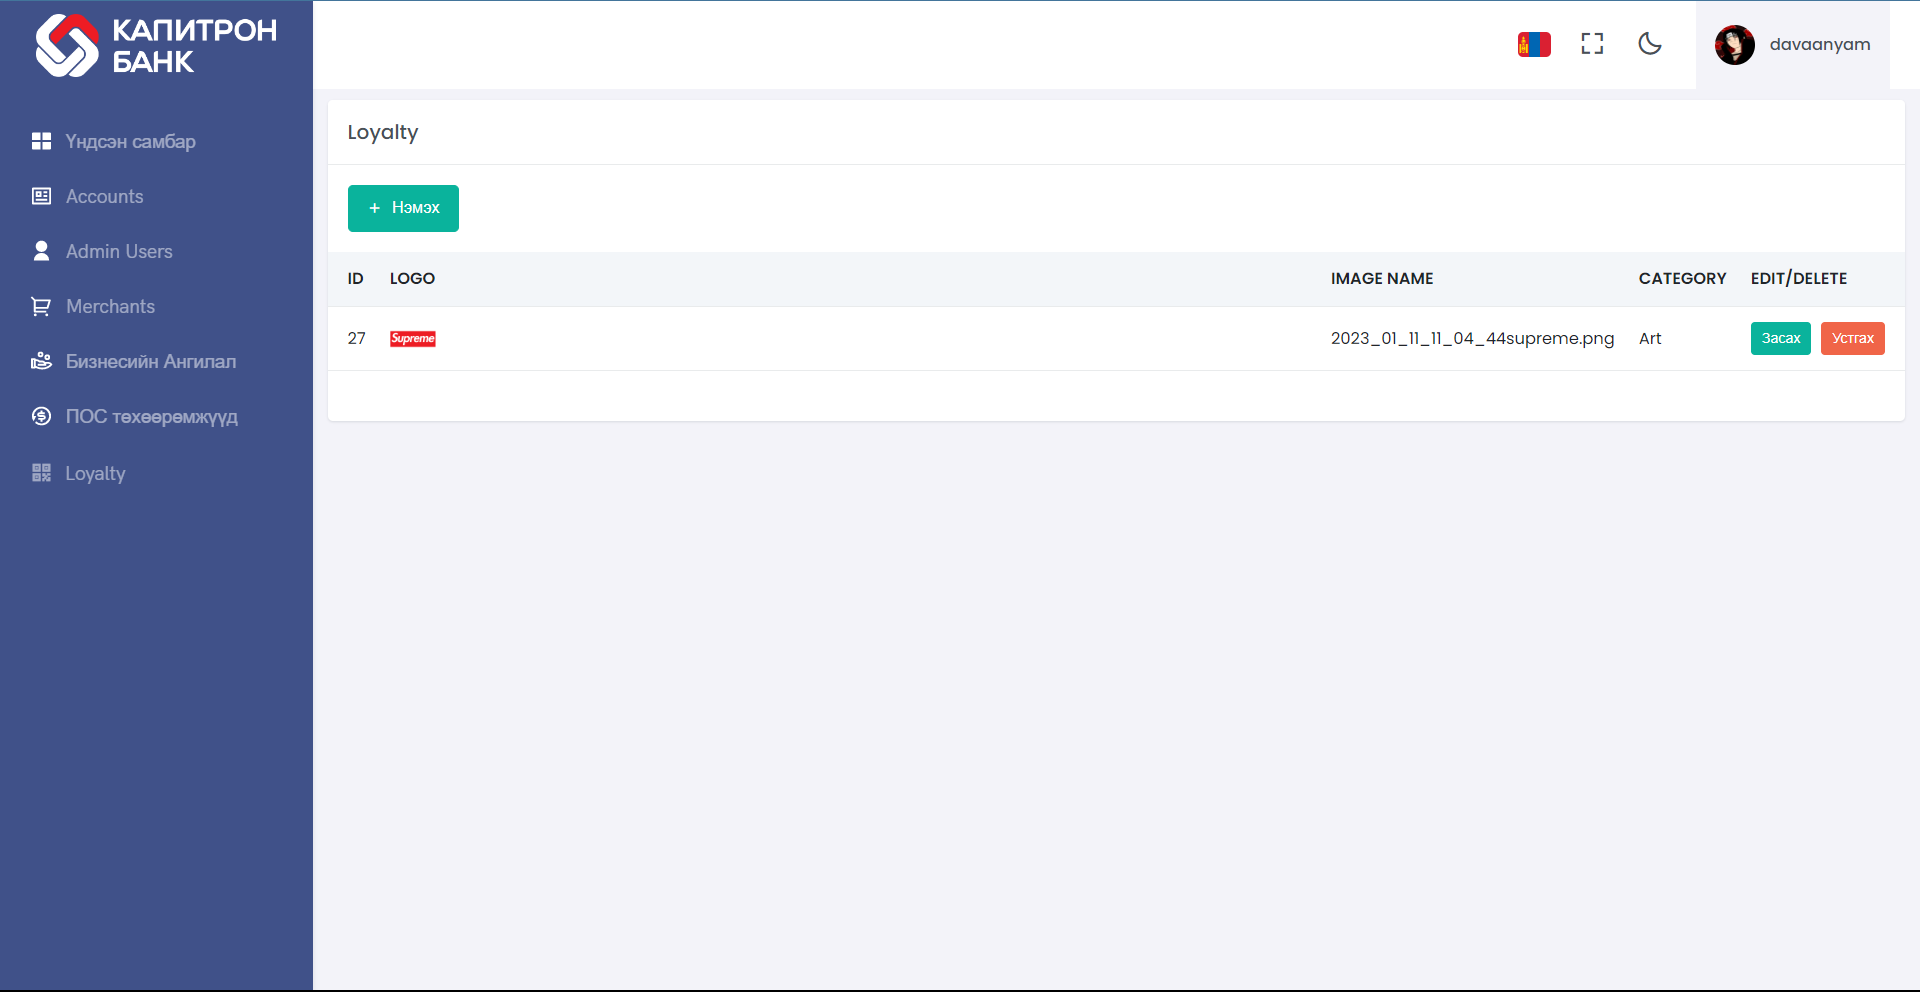
\includegraphics[width=15cm]{images/crud.png}
	\caption{Loyalty CRUD}
	\label{fig:toast}
\end{figure}
\pagebreak
\begin{figure}
	\centering
	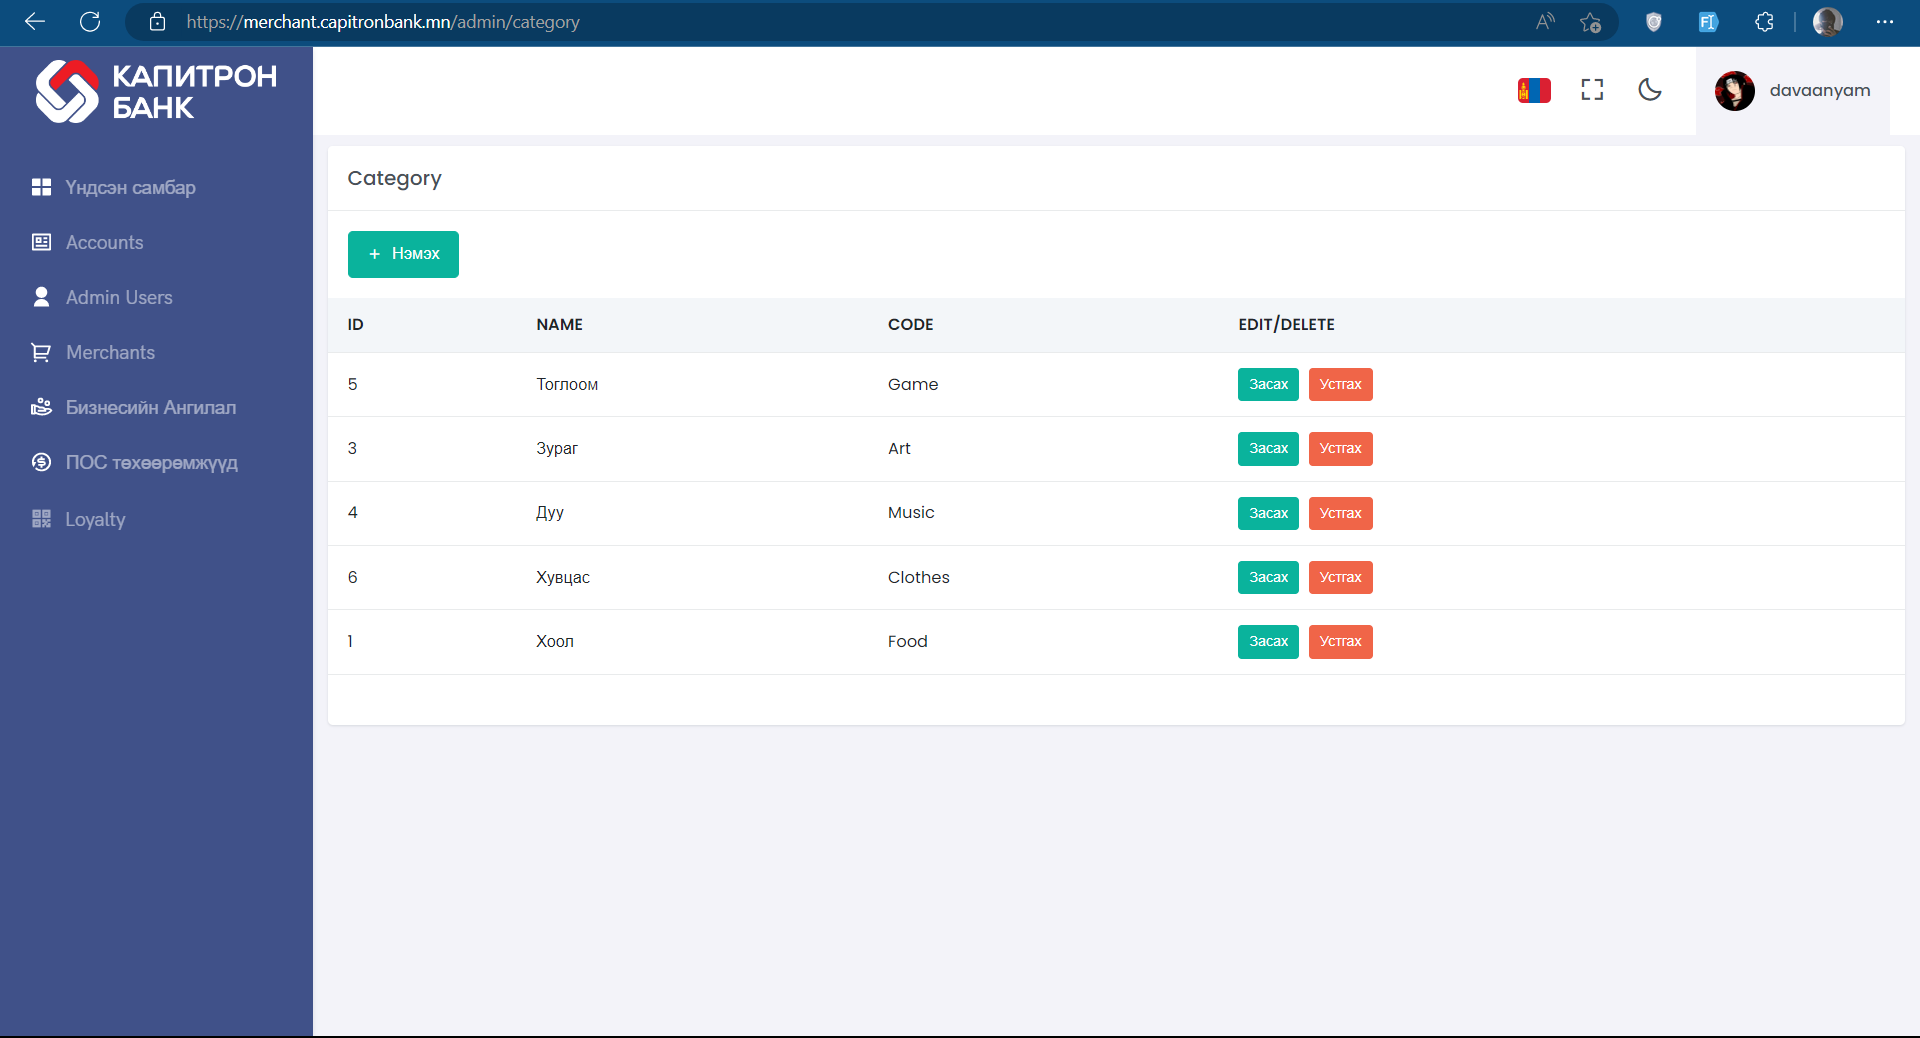
\includegraphics[width=15cm]{images/crud1.png}
	\caption{Loyalty Category CRUD}
	\label{fig:toast}
\end{figure}
\pagebreak
\pagebreak
\section{Үр дүнгийн тайлан}
Миний бие "Капитрон банк"-д 24 хоногийн хугацаатай дадлага хийх үеэр би Laravel PHP framework, jQuery, AJAX ашигласан төсөл дээр ажиллах боломж олдсон. Энэ туршлагаараа би хэрэглэгчдэд ээлтэй динамик вэб програмуудыг хэрхэн бүтээх талаар илүү гүнзгий ойлголттой болж. Laravel-ийн үндсийг болон түүний route, blade template, Equolent ORM зэрэг хүчирхэг функцуудыг сурав. Мөн jQuery болон AJAX-тай ажиллах туршлага хуримтлуулсан бөгөөд энэ нь вэбсайтад интерактив элементүүдийг нэмж, илүү динамик, үр дүнтэй болгох арга барилуудыг амжилттай эзэмшсэн гэж дүгнэж байна. Мөн төсөл дээр ажиллах боломж олгосон баг, зааварчилгаа өгч байсан ахлахдаа талархаж байна.

\quad Нэмж дурдахад би энэ төсөл дээр ажиллаж байхдаа олж авсан бодит туршлагаараа технологиуд хэрхэн хоорондоо нэгдэж, үр дүнтэй вэб програмыг бий болгохыг сурж, ур чадвараа цаашдын төслүүдэд үргэлжлүүлэн хэрэгжүүлэхдээ баяртай байна.